\chapter{Ergebnisse} \label{sec:results}


\subsubsection{Mittlere Szenarien}



Die Messungen haben ergeben, dass für alle mittelgroßen Szenarien $s \in S_{Anon_M}$ gilt, dass $t_{sub_{MatFlowG}}(s) < t_{sub_{IdObj}}(s)$. Hierbei haben sich für Identical Objects die Laufzeiten über die 13 Szenarien von $S_{Anon_M}$ zwischen 11s und 1min 39s bewegt, während die Laufzeiten von Material Flow Graph zwischen 1s und 9s lagen. Mit $p=2,744 \cdot 10^{-9}$ ist Material Flow Graph \textit{statistisch signifikant} schneller\footnote{Einseitiger Zwei-Stichproben-t-Test mit unterschiedlicher Varianz; Normalverteilung angenommen; $n=12$; Szenario $z$ mit $t_{sub_{IdObj}}(z) = 1min 39s$ und $t_{sub_{MatFlowG}}(z) = 9s$ als Ausreißer von Test exkludiert.}. 

\begin{table}[ht]
	\centering
	\begin{tabular}{l|l|l|l|l}
		Szenario & $t_{sub_{IdObj}}$ & $t_{sub_{IdMat}}$& $t_{sub_{MatFlowG}}$ & $f_{IdObj \rightarrow MatFlowG}$ \\
		\midrule
		$s_{Krit}$ & 9h 41min 20s & 14min 47s & 3min 31s & $168,15$ \\
		$s_{Ult}$ & 21h & 2h 45min & 15min & $83,\bar{3}$ \\
		
	\end{tabular}
	\caption{Ergebnisse der Laufzeitmessungen von $S_L$ nach verschiedenen Methoden. Außerdem der Beschleunigungsfaktor $f$ von Identical Objects zu Material Flow Graph. Szenario $s_{Ult}$ wurde auf einem Server durchgeführt (Speicherbedarf zu hoch), $s_{Krit}$ auf dem in \autoref{sec:rahmen} beschriebenen Rechner.}
	\label{tab:large_scenarios}
\end{table}

\begin{table}[ht]
	\centering
	\begin{tabular}{l|l|l|l}
		$S_X$ & $\bar{m}_{pre}$ & $\bar{m}_{post}$& $f$ \\
		\midrule
		small & $45,11$ & $5,94$ & $7,6$ \\
		medium & $395,82$ & $120,3$ & $3,29$ \\
		large & $4711,24$ & $50,01$ & $94,19$ \\
	\end{tabular}
	\caption{Durchschnittliche Knotenanzahl vor der Graphenreduktion $\bar{m_{pre}}$, nach der Graphenreduktion $\bar{m_{post}}$ und deren mittlerer Reduktionsfaktor $f$ nach Szenario-Klassen.}
	\label{tab:scenarios_node_nb}
\end{table}

\begin{figure}
	\centering
	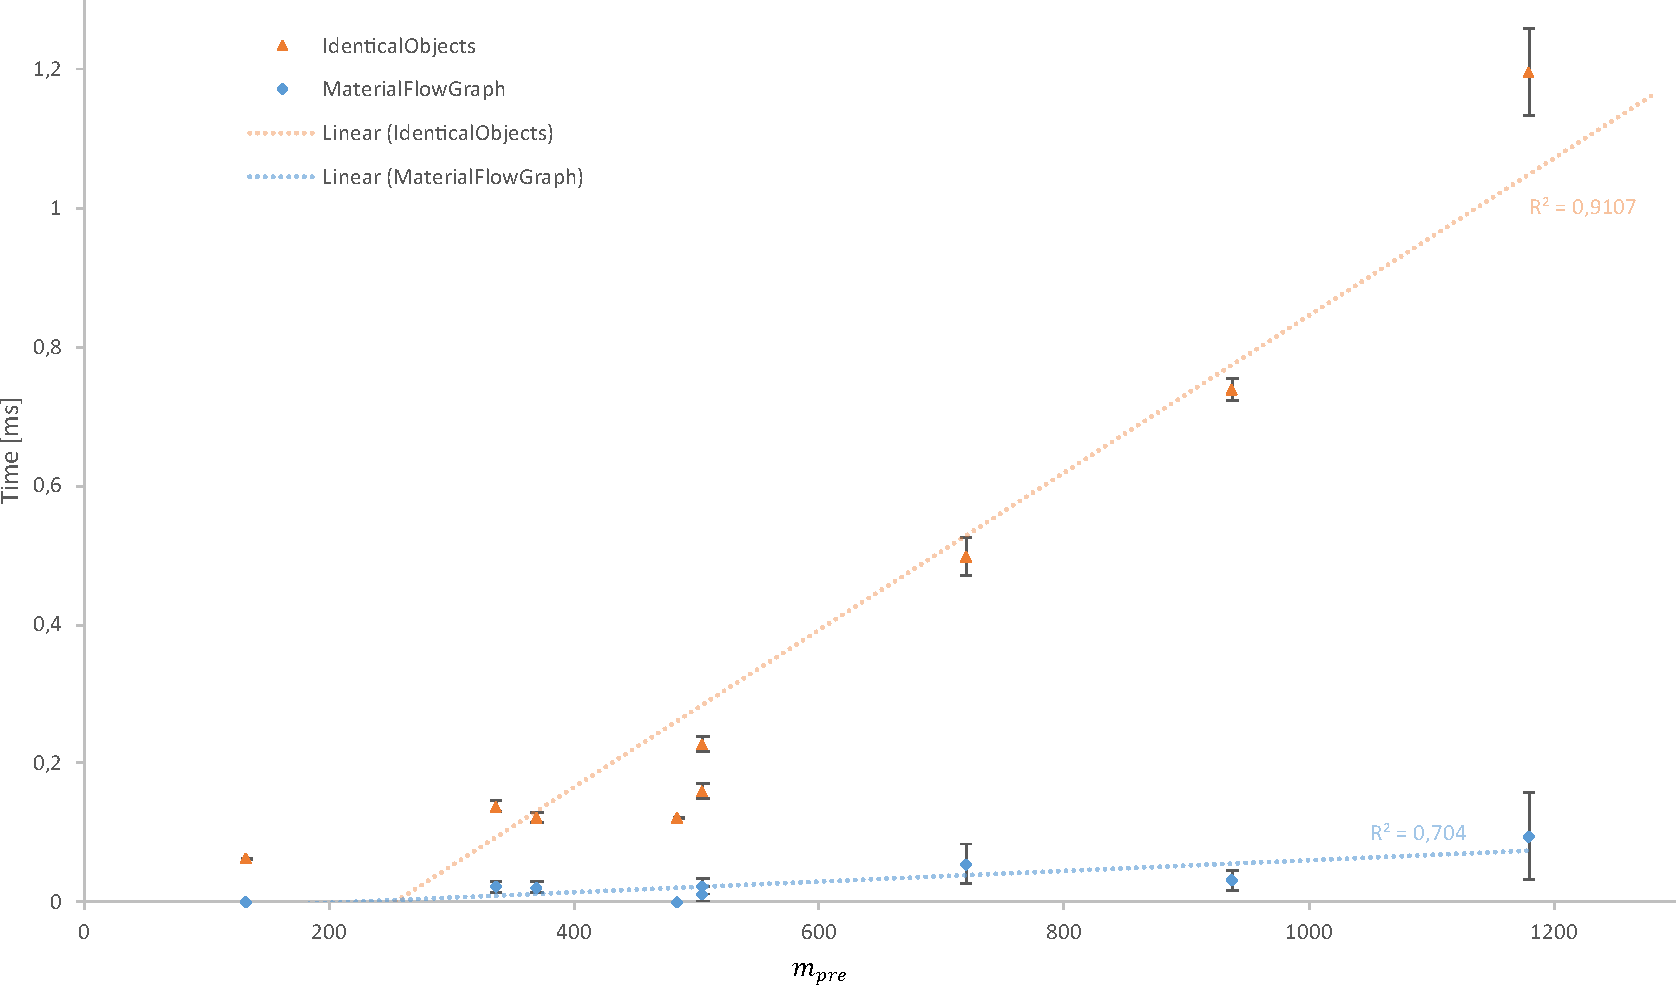
\includegraphics[width=1.00\textwidth]{Bilder/performance_per_comp.pdf} 
	\caption{Mittlere Graphengröße $m$ mittelgroßer Szenarien abgebildet auf die durchschnittliche Laufzeit von $t_{sim}$ in $ms$ nach Identical Objects (orange), Material Flow Graph (blau) mit Trendlinien nach linearer Regression.}
	\label{fig:time_comp}
\end{figure}

Abschließend zur Untersuchung der praktischen Tests lässt sich also festhalten, dass die erwarteten Ergebnisse erzielt, sowie die theoretischen Überlegungen praktisch bestätigt werden konnten.